% begin module fermats-theorem
\begin{frame}
\frametitle{Fermat's Theorem}
The next theorem gives a condition that can help to find local maxima and minima.
\end{frame}

\begin{frame}[t]
\begin{theorem}[Fermat's Theorem]
Let $f$ be a function defined in an open interval around $c$ and such that  \alert<handout:0| 11,18>{$f'(c)$ exists}. If $f$ has a local maximum or minimum at $c$, then $f'(c) = 0$.
\end{theorem}
\begin{proof}
\begin{itemize}
\item<2->  We will prove the case when $f$ has a local maximum at $c$.
\item<3->  This means that $f(x) \leq f(c)$ for all $x$ close to $c$.
\item<4->  If $h$ is very small (negative or positive), then \uncover<4->{%
$f(c + h) - f(c) \leq 0$.
}%
\item<5->  Suppose $h$ is positive, and divide both sides by $h$:
\abovedisplayskip=0pt
\belowdisplayskip=0pt
\[
\uncover<11->{%
\alert<handout:0| 11>{\alert<handout:0| 19>{f'(c)} = \lim_{h\to 0}} %
\alert<handout:0| 11>{\frac{f(c + h) - f(c)}{h}= } %
}%
\uncover<7->{%
\alert<handout:0| 7,10-11>{\lim_{h\to 0^+}} %
}%
\uncover<6->{%
\alert<handout:0| 10-11>{\frac{f(c + h) - f(c)}{h}} \alert<handout:0| 19>{\leq} %
}%
\uncover<7->{%
\alert<handout:0| 7-9>{\lim_{h\to 0^+}} %
}%
\uncover<6->{%
\alert<handout:0| 8-9>{0} %
}%
\uncover<9->{%
\alert<handout:0| 8-9>{= \alert<handout:0| 19>{0}} %
}%
\]
\item<12->  Suppose \alert<handout:0| 13>{$h$ is negative}, and divide both sides by $h$:
\abovedisplayskip=0pt
\belowdisplayskip=0pt
\[
\uncover<18->{%
\alert<handout:0| 18>{\alert<handout:0| 20>{f'(c)} = \lim_{h\to 0}} %
\alert<handout:0| 18>{\frac{f(c + h) - f(c)}{h}= } %
}%
\uncover<14->{%
\alert<handout:0| 14,17-18>{\lim_{h\to 0^-}} %
}%
\uncover<12->{%
\alert<handout:0| 17-18>{\frac{f(c + h) - f(c)}{h}} \alert<handout:0| 13,20>{\geq} %
}%
\uncover<14->{%
\alert<handout:0| 14-16>{\lim_{h\to 0^-}} %
}%
\uncover<12->{%
\alert<handout:0| 15-16>{0} %
}%
\uncover<16->{%
\alert<handout:0| 16>{= \alert<handout:0| 20>{0}} %
}%
\]
\item<19->  Therefore \alert<handout:0| 19>{$f'(c) \leq 0$} \uncover<20->{and \alert<handout:0| 20>{$f'(c) \geq 0$}}\uncover<21>{, so \alert<handout:0| 21>{$f'(c) = 0$}.}\qedhere
\end{itemize}
\end{proof}
\end{frame}


\begin{frame}[t]
\begin{theorem}[Fermat's Theorem]
Let $f$ be a function defined in an open interval around $c$ and such that $f'(c)$ exists. If $f$ has a local maximum or minimum at $c$, then $f'(c) = 0$.
\end{theorem}
\begin{center}
\psset{xunit=1cm, yunit=1cm}
\begin{pspicture}(-5, -5)(5,5) 
\tiny
\psframe*[linecolor=white](-5,-5)(5,5) 
\psaxes[ticks=none, labels=none]{<->}(0,0)(-0.5,-0.5)(5.5,4.5)
%Function formula: -1/2 ((x)^{2})+1/15 ((x)^{3})+5/2+9/20 (x) 
\psplot[linecolor=red, plotpoints=1000]{0}{5.5}{x 0.45 mul 2.5 add x 3 exp 0.0666667 mul add x 2 exp -0.5 mul add }
\psFullDotBlue{0.5}{2.60833}
\rput[b](0.5, 2.80833){$(c,f(c)) $}
\psline[linecolor=blue](0.1,2.60833)(0.9,2.60833)
\psline[linestyle=dashed](0.5, 0)(0.5, 2.60833)
\psline(0.5, -0.1)(0.5, 0.1)
\rput[t](0.5, -0.2){$c$}

\psFullDotBlue{4.5}{0.475}
\rput[b](4.5, 0.675){$(d,f(d)) $}
\psline[linecolor=blue](4.1,0.475)(4.9,0.475)
\psline[linestyle=dashed](4.5, 0.475)(4.5, 0)
\psline(4.5, -0.1)(4.5, 0.1)
\rput[t](4.5, -0.2){$d$}

\end{pspicture} 
%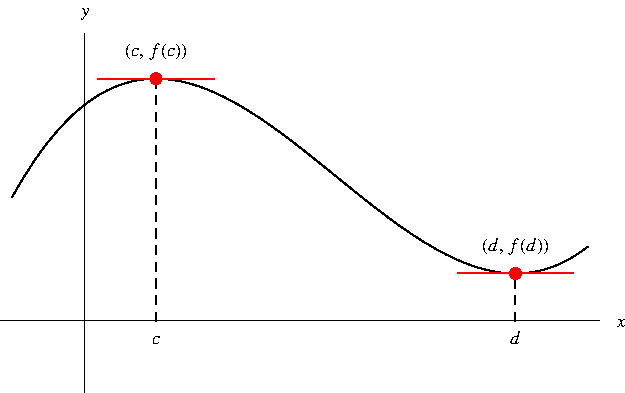
\includegraphics[width=10cm]{maxima-minima/pictures/04-01-ferm.pdf}%
\end{center}
\end{frame}
% end module fermats-theorem
